%% part1
\MinParskip{}

\section{Basic Introduction}

\subsection{Background}
Light pollution is a term used to describe the excessive or inappropriate use of artificial light, which can take the form of light trespass, over-illumination, and light clutter. These phenomena are often visible as a glow in the night sky in large cities, but they can also occur in more remote areas. Light pollution affects our environment, health, and safety by altering our view of the night sky, delaying or accelerating plant maturation, disrupting wildlife migration patterns, and affecting our circadian rhythms. Excessive artificial light can lead to poor sleep quality and may contribute to physical and mental health problems, while glare from artificial lights can increase the risk of motor vehicle accidents.

However, artificial light has both positive and negative impacts that can vary based on location. The effects of light pollution can depend on factors such as a location's level of development, population, biodiversity, geography, and climate. Therefore, assessing the extent of the effects and potential impacts of intervention strategies must be tailored to the specific location, and intervention strategies are needed to mitigate the negative effects of light pollution.

\subsection{Problem Restatement}
\begin{itemize}
    \item The indicators of the EWM-TOPSIS model should be determined, in other words, it is equal to build a broadly applicable metric for identifying the light pollution risk level.
    \item Apply the indicators and the related data to the EWM-TOPSIS model, then analyse the result in the four diverse types of locations.
    \item Design 3 possible strategies for addressing light pollution, and how the indicators change with the strategies.
    \item Select 2 locations, and implement the most effective intervention strategies for each of them. See how the indicators change and the impact of the chosen intervention strategy.
    \item Write a 1-page flyer to community officials or local groups in a specific location to promote its most-effective intervention strategy.
\end{itemize}

\subsection{Our works}
    \cite{LBMA}
    \begin{figure}\centering
        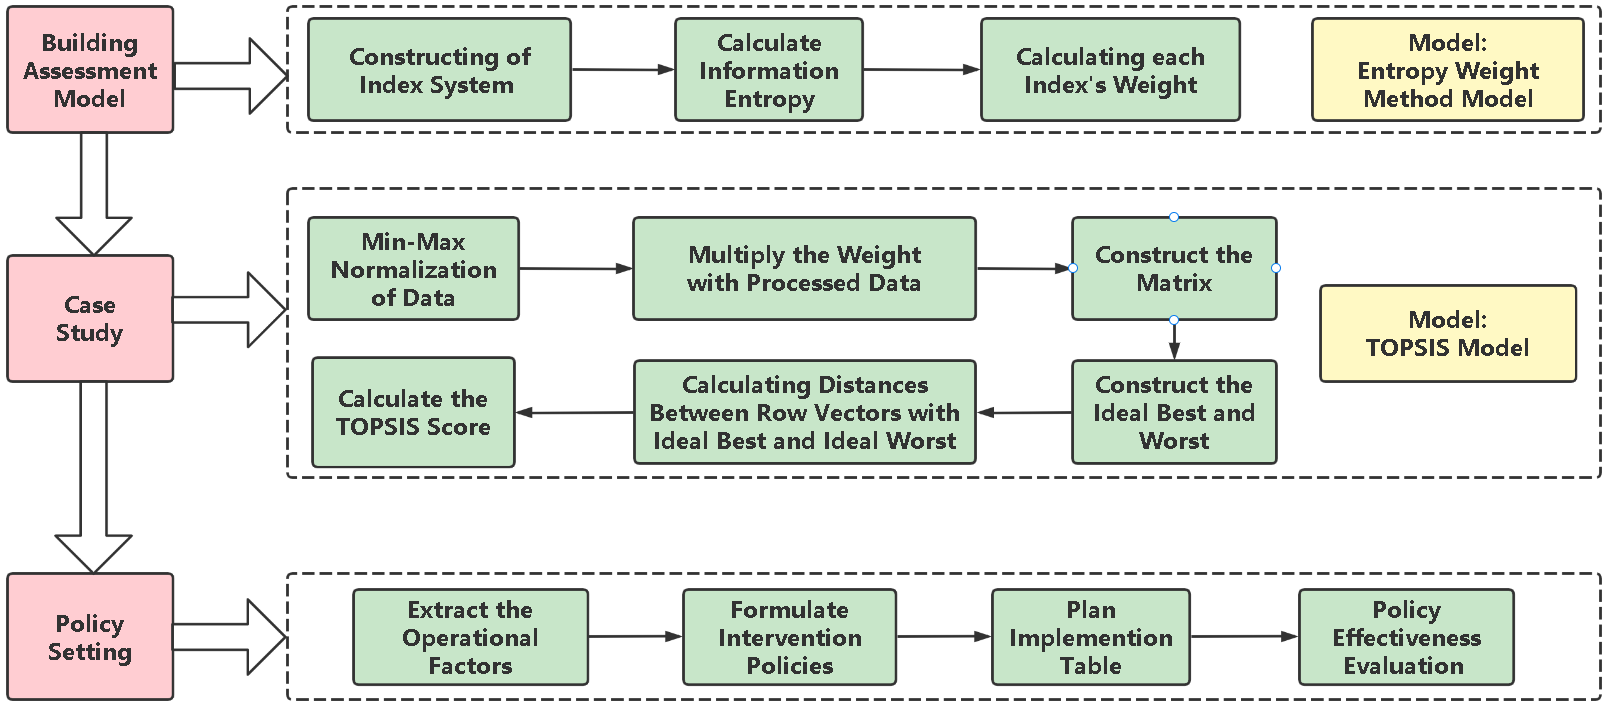
\includegraphics[width=1\textwidth]{figures/Flowchart}
        \caption{Our workflow.} \label{fig:figure1}
    \end{figure}



